%===============================================================================
\section{Introduction}
\label{sec:intro}
	 
In open-ended real-world environments, the right tool is rarely at hand, yet humans adapt effortlessly by repurposing available objects to accomplish functions. For example, in hitting, a book, a stone, or a shoe can be used to drive a nail because functionally equivalent tools share a common functional intent: a contact region to strike with and a motion that brings it onto the target. 
This capacity, which we term \textit{functional generalization}, is a hallmark of human dexterity that robots have yet to achieve. Current manipulation policies overfit to the appearance and geometry of seen tools, failing when handed a novel one that serves the same function~\citep{chen2025tool, turpin2021gift, qin2023robot, jia2026action, bai2026flash}.

\begin{figure}[ht]
    \centering
    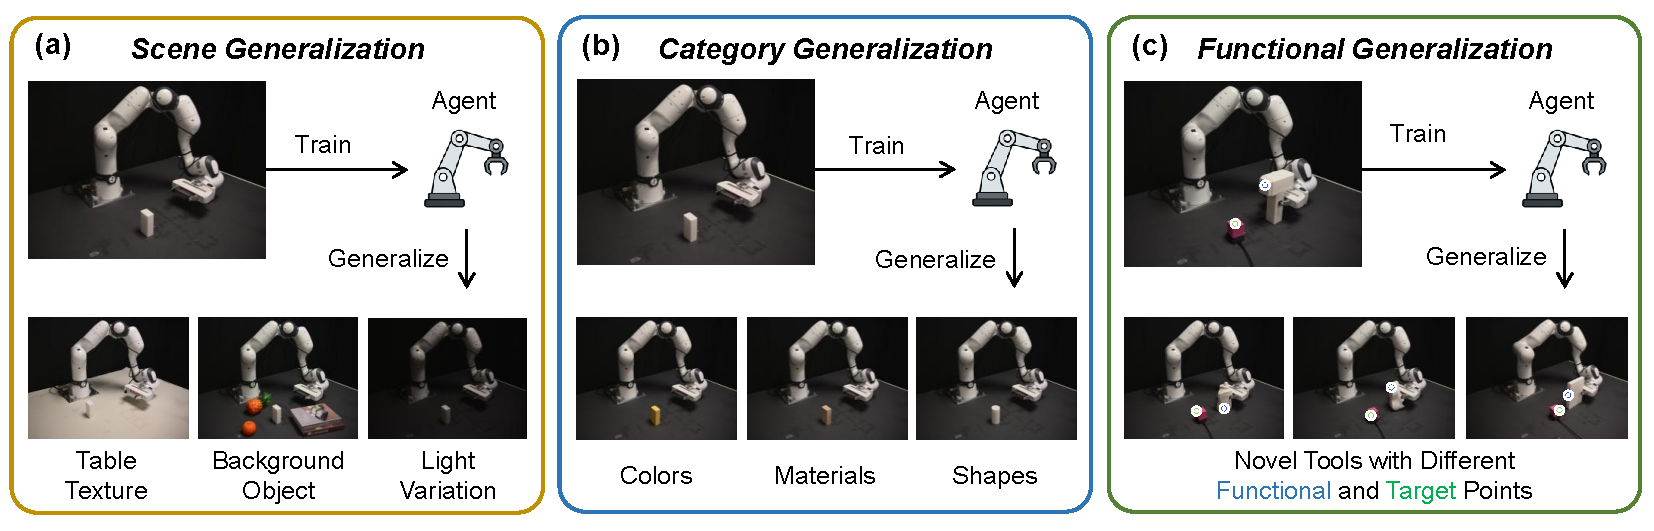
\includegraphics[width=1.0\linewidth]{figures/teaser_v2.pdf}
    % \caption{
    % \textbf{Comparison between functional generalization and existing generalization settings.}
    % (a) Scene generalization evaluates robustness to visual variations.
    % (b) Category generalization tests transfer across objects with diverse properties.
    % (c) Functional generalization requires using unseen tools to accomplish the same function.
    % }
    \caption{
    \textbf{Comparison of functional generalization with existing generalization settings.}
    (a) Scene generalization handles visual variations.
    (b) Category generalization transfers across object properties.
    (c) Functional generalization uses unseen tools for the same function.
    }
    \label{fig:functional_generalization}
\end{figure}
Functional generalization is fundamentally harder than conventional generalization. As illustrated in Fig.~\ref{fig:functional_generalization}, scene- and category-level generalization require tolerating visual variations while the underlying motion stays the same~\citep{goyal2023rvt, shridhar2023perceiver, shridhar2022cliport, nair2023r3m}. Functional generalization, by contrast, {demands adapting the motion to each tool's geometry}: striking a target with a novel tool requires locating its contact region, aligning it, and producing an appropriate motion, even when the tool's shape and required trajectory differ from training. {The core difficulty is a mismatch: functionally equivalent tools exhibit common functional intent that can be perceived from visual observations, but realizing the same function requires different motions across tools.}


%Bridging this perception-to-action gap requires an intermediate representation that carries functional intent across tools, satisfying two competing demands:  expressive enough to capture where to make contact and how to move onto the target, yet grounded enough to be predicted from \textcolor{cBlue}{perceived} observations without overfitting to tool-specific appearance. 
Bridging this perception-to-action gap requires an intermediate representation that carries functional intent across tools, satisfying two competing demands: {it should be expressive enough to capture where contact can occur and how a selected contact region should move toward the target, yet abstract enough to discard tool-specific appearance that may hinder generalization to unseen tools.}
Dense representations like raw video entangle function-relevant cues with tool-specific appearance, while overly sparse ones discard the geometric and temporal structure needed for precise action grounding. This trade-off raises the central question of our work: \textit{which representation best transfers functional intent from perception to action?}

To answer this question, we evaluate intermediate representations 
including affordance images, human video prompts, {functional videos and object masks}, and 2D keypoint trajectories, 
finding that keypoint trajectories best balance functional expressiveness and 
action groundability: they capture function-relevant contact and motion structure 
while discarding tool-specific appearance that causes overfitting. Building on 
this, we propose \algoname{}, a two-stage framework that 
decouples functional reasoning from action execution.
%it first predicts  generalizable keypoint trajectories for unseen tools from large-scale action-free data, then grounds these functional plans into executable robot actions using a small set of action-labeled demonstrations. 
{It learns a functional keypoint predictor from large-scale action-free data and an action-grounding policy from limited action-labeled demonstrations. At inference, the predictor predicts function-relevant keypoint trajectories, which the execution policy grounds into robot actions.
We further introduce a benchmark spanning ten tools and three functions, including hitting, sweeping, and hooking, on which \algoname{} consistently outperforms state-of-the-art methods on unseen tools in both simulation and the real world, achieving substantial gains in average success rate.}
In summary, our contributions are threefold:
\begin{itemize}[leftmargin=*]
    \item We formalize \textit{functional generalization} in robotic tool-use and identify the perception-to-action gap as its core difficulty.
    \item We find that 2D keypoint trajectories best balance functional 
    expressiveness and action groundability, and propose \algoname{}, {a two-stage framework that learns functional keypoint planning from action-free data and action grounding from limited robot demonstrations.}
    % \textcolor{cBlue}{\item Through extensive simulation experiments across 10 tools and three functions, together with real-world validation, we demonstrate that \algoname{} consistently outperforms state-of-the-art methods on unseen tools.}
   {\item Across ten tools and three functions in simulation, with real-world validation, we demonstrate that \algoname{} consistently outperforms state-of-the-art methods on unseen tools.}
\end{itemize}


